\documentclass[12pt]{amsart}
\usepackage{geometry}
\usepackage{amsmath}
\usepackage{amssymb}
\usepackage{graphicx}
\usepackage{subfig}
\usepackage[table]{xcolor}
\usepackage{color}
\usepackage{natbib}

\usepackage{blindtext}
\usepackage{tabularx}

\newenvironment{frcseries}{\fontfamily{frc}\selectfont}{}
\newcommand{\textfrc}[1]{{\frcseries#1}}
\newcommand{\mathfrc}[1]{\raisebox{-0.8mm}{\text{\textfrc{\small #1}}}\hspace{0.4mm}}


\geometry{letterpaper}



% general commands
\definecolor{lemonchiffon}{rgb}{1, .98, .80}
\definecolor{lightgrass}{rgb}{.89, 1, .87}
\newcommand{\vect}[1]{\boldsymbol{\mathbf{#1}}}
\newcommand{\degree}[1]{${#1}^{\circ}$}
\newcommand{\highlight}{ \rowcolor{lightgrass} }
\newcommand{\script}[1]{\mathcal{#1}}

\newcommand{\eqn}[1]{\begin{align*}
#1
\end{align*}}
\newcommand{\eqnl}[2]{\begin{align} \label{#1}
#2
\end{align}}
\newcommand{\shblock}{\hspace{3mm}}
\newcommand{\hblock}{\hspace{8mm}}
\newcommand{\eqnsep}{\shblock\hblock}

\newcommand{\bl}{\big\{}
\newcommand{\br}{\big\}}
\newcommand{\Bl}{\Big\{}
\newcommand{\Br}{\Big\}}

\newcommand{\argmax}{\operatornamewithlimits{argmax}}

\newcommand{\indicator}{\mathbf{1}}

\newcommand{\mtx}[4]{
\[
#1 = #2
\left[ {\begin{array}{#3}
 #4
 \end{array} } \right]
\]
}

\newcommand{\eqnset}[4]{
\[ #1 = #2 \left\{ \begin{array}{#3}
        #4
\end{array} \right. \] 
}



        
        
        
        \newcommand{\img}[2]{
	\begin{figure}
		\centering
		\includegraphics[width=\textwidth]{#1}
		\caption{#2}
	\end{figure}
}

\newcommand{\imgi}[1]{
	\vspace{10mm}
	\includegraphics[width=\textwidth]{#1}
	\vspace{10mm}
}


% paper specific terms
\newcommand{\vz}{\vect{z}}
\newcommand{\vx}{\vect{x}}
\newcommand{\vy}{\vect{y}}
\newcommand{\vp}{\vect{\pi}}
\newcommand{\vph}{\hat{\vect{\pi}}}
\newcommand{\vpmle}{\hat{\vect{\pi}}_\text{MLE}}



\newcommand{\fab}{f_j}
\newcommand{\llp}{\mathfrc{l}(\vect{\pi})}

\newcommand{\pims}{1-\pi_1,\ldots,\pi_{m-1}}

\newcommand{\hessll}[2]{\sumn \frac{f_{#1}}{(\summ \pi_j f_j)^2 f_{#2}}}
\newcommand{\hessllg}[2]{\sumn \frac{f_{#1}}{(\sumg \pi_j f_j)^2 f_{#2}}}
\newcommand{\hesslld}[2]{\frac{\partial^2 \llpp}{\partial \pi_{#1} \partial \pi_{#2}}}


\newcommand{\sumn}{\sum^n_{i=1}}
\newcommand{\summ}{\sum^m_{j=1}}
\newcommand{\summo}{\sum^{m-1}_{j=1}}
\newcommand{\sumg}{\sum^g_{j=1}}
\newcommand{\sumk}{\sum^m_{k=1}}

\newcommand{\vpg}{\vp^{\prime}}
\newcommand{\vpgh}{\hat{\vp}^{\prime}}
\newcommand{\llpp}{\mathfrc{l}(\vpg)}
\newcommand{\llpph}{\mathfrc{l}(\vpgh)}


%%% TITLE
\title{Metallicity}
\author{\today}

%%% BEGIN DOCUMENT
\begin{document}

\maketitle






%%%%%%%%%%%%%%%%%%%%%%%%%%%%%%%%%%%%%%%%%%%%%%%%%%%%%%
\section{Mixture model}

Given $n$ observed $(\frac{\alpha}{\text{Fe}}, \frac{\text{Fe}}{\text{H}})$ metallicities as $\bl (x_i,y_i) \br^n_{i=1}$, or as $(\vx,\vy)$, each of which is drawn from one of $m$ known model densities, we model the density of observations using the mixture model

\eqnl{mixmodel}{
	f(x,y) = \summ \pi_j \fab(x,y)
}

where \eqn{
	\summ \pi_j = 1 \eqnsep \pi_j \geq 0, \hspace{3mm} j=1,\ldots,m
 }

From the summation constraint, $\vp$ has $m-1$ free parameters: \eqn{
	\vp = (\pi_1, \ldots, \pi_{m-1}, 1-\pi_1-\ldots-\pi_{m-1})
}

Thus the likelihood of \eqref{mixmodel} is

\eqn{
	L(\vect{\pi}) &= \prod^n_{i=1} f(x_i,y_i)	 \\
	&= \prod^n_{i=1} \Bl  \summ \pi_j \fab(x_i,y_i)  \Br	\\
	\log L(\vect{\pi}) &= \sumn \log \Big( \summ \pi_j \fab(x_i,y_i)  \Big)
}

Maximizing $\log L(\vect{\pi})$ with respect to $\vp$ will yield $\vpmle$, but this arduous task can be avoided by adding a latent indicator, $z$, to the observed data $(\vx, \vy)$, representing the model group from which that observation was generated. Let $G_j$ be the $j^\text{th}$ model group, and let

\eqn{z_{ij} = \indicator \bl (x_i,y_i) \mapsto G_j \br}


The complete data likelihood is defined over the complete data $\bl (x_i,y_i,\vect{z}_i) \br^n_{i=1}$ as

\eqn{
	L(\vect{\pi}) &= \prod^n_{i=1} \prod^m_{j=1} \Bl \fab(x_i,y_i) \Br ^{z_{ij}} \pi_j^{z_{ij}}
}
\eqnl{loglike}{
	\llp &= \sumn \summ z_{ij}  \log \bl \pi_j  \fab(x_i,y_i) \br
}





%%%%%%%%%%%%%%%%%%%%%%%%%%%%%%%%%%%%%%%%%%%%%%%%%%%%%%

\section{Expectation Maximization}

One way to estimate $\vp$ is to use a maximum likelihood estimate, $\vph$, computed using expectation maximization. Starting from an initial set of guesses, $\vp^{(0)}$, we iteratively find the expected value of the likelihood, \eqref{loglike}, conditional on the data, and then find the $\argmax_{\vp}$ of this expectation. The maximizing value the $t^\text{th}$ iteration, $\vph^{(t)}$, is then used as the starting value for the next run, and we continue until the likelihood changes by less than $10^{-3}$ over twenty five iterations.

\subsection{Expectation step}
First we find the expected value of the log likelihood, \eqref{loglike}, conditional on the data. Note that since $z_{ij}$ is an indicator function, its expected value is equal to the probability that data point $i$ comes from model $j$.

\eqnl{estep}{
	\text{E}_{\vp}\Big[\llp \big| \vx,\vy \Big] &= \sumn \summ \text{E}_{\vp}\big[z_{ij}|x_i,y_i\big] \bl \log \fab(x_i,y_i) + \log \pi_j  \br
}

Since we're ultimately maximizing, the non-constant component is of primary interest, and can be analytically specified by applying Bayes' rule:
\eqn{
	\text{E}_{\vp}\Big[  z_{ij} | x_i, y_i \Big] &= \text{Probability}\Big((x_i,y_i) \mapsto G_j \big | x_i,y_i\Big)	\\
	&= \text{Pr}_{\vp}(z_{ij}|x_i,y_i)	\\
	&= \frac{p(x_i,y_i|z_{ij}=1)p(z_{ij}=1)}{p(x_i,y_i)}	\\
}

Thus the expected value of the indicator variable, $z_{ij}$, given the data and the parameters, $\vp$, of the data's distribution defined by \eqref{mixmodel} is
\eqnl{expstep}{
	\text{E}_{\vp}\Big[  z_{ij} | x_i, y_i \Big] &=  \frac{\pi_j \fab(x_i,y_i)  }{\summ \pi_j \fab(x_i,y_i)}
}
%The expectation maximization algorithm is iterative, and so, when evaluating, the $\vp$ above comes from the $\argmax_{\vp}$ prior iteration.

To iteratively evaluate this expectation, we let $w^{(t)}_{ij}$ be \eqref{expstep} at the $t^\text{th}$ step:
\eqnset{w^{(t+1)}_{ij}}{}{ll}{
	\frac{\displaystyle\pi^{(t)}_{j} \fab(x_i,y_i)}{\displaystyle\sumk \pi^{(t)}_{k}f_k(x_i,y_i)}				& j=1,\ldots,m-1	\\
	\vspace{1mm} & \\
	1 - w_{i1} - \ldots - w_{i,m-1}		& j=m
}

Since $\vp$ is not defined for the first evaluation, we use a random initialization to generate $\vect{w}_{j}^{(0)}$. Convergence is not sensitive to the choice of values in this case, but may be if the likelihood is riddled with local maxima.

\subsection{Maximization step}
We now have an explicit formulation for the expected log likelihood \eqref{expstep} given a single parameter $\vp$, plus the data. The argument of the maximum of \eqref{expstep} at each iteration $t$ provides an estimate that approaches the MLE of $\vp$, and is given by:

\eqnl{argmaxpi}{
	\vph^{(t)} &= \argmax_{\vp} \text{E}\Big[\llp \big| \vx,\vy,\vph^{(t-1)} \Big]   
}

Accounting for the $m-1$ free parameters of $\vp$, differentiation of \eqref{expstep} proceeds, for $k=1,\ldots,m-1$, as:

\eqn{
	\frac{\partial}{\partial \pi_k} \text{E}\Big[\llp \big| \vect{x},\vect{y}\Big]   &=      \sumn \Bl  w^{(t-1)}_{ik} \frac{1}{\pi_k} - w^{(t-1)}_{im} \frac{1}{1-\pi_1-\ldots-\pi_{m-1}}   \Br
}
\eqn{
	\frac{1}{\pi_k} \sumn w_{ik}^{(t-1)} &= \frac{1}{1-\pi_1-\ldots-\pi_{m-1}} \sumn w_{im}^{(t-1)}
}

Consequently, using some constant, $c$, we must have
\eqn{
	\frac{1}{\pi_k} \sumn w^{(t-1)}_{ik} &= \ldots = \frac{1}{\pi_{m-1}} \sumn w^{(t-1)}_{i,m-1} = c	\\
	\hat{\pi}_k^{(t)} &= \frac{\sumn w^{(t-1)}_{ik}}{c}
}

The unknown constant $c$ appears problematic, but, because $\summ \pi_j = 1$, algebraic manipulation reveals that $c=n$, yielding a final solution that can be numerically evaluated:
\eqn{
	\hat{\pi}^{(t)}_k &= \frac{\sumn w^{(t-1)}_{ij}}{n}	\\
	\hat{\pi}^{(t)}_m &= 1-\pi_1-\ldots-\pi_{m-1}
}

In our case, computation of $\vph$ converges relatively quickly for all starting values: on the order of 600 iterations, or half a minute, for our stopping criteria. Large $\pi_k$ values typically emerge after two or three iterations, and most change, absolutely speaking, occurs in the first fifty to one hundred iterations.


















%%%%%%%%%%%%%%%%%%%%%%%%%%%%%%%%%%%%%%%%%%%%%%%%%%%%%%
\clearpage
\section{Covariance and correlation of $\vph$}
The asymptotic covariance matrix of $\vph$ can be approximated by the inverse of the observed Fisher information matrix, $I$.

As $\pi_m = 1-\sum_{j=1}^{m-1}\pi_j$, there are only $m-1$ free parameters. Thus let $\vpg=(\pi_1,\ldots,\pi_{m-1})$. Using $f_{ij} = f_j(x_i,y_i)$ for brevity, the likelihood can then be expressed as:
\eqnl{llinfo}{
	\llpp &= \sumn \log \Bigg\{ \Big( \summo \pi_{j} f_{ij} \Big) + (\pims)f_{im} \Bigg\}	
}



The observed information matrix, $I$, is the $m-1\times m-1$ negative hessian of \eqref{llinfo}, evaluated at the observed data points:

\mtx{I(\vpg|\vx,\vy)=-\frac{\partial^2 \llpp}{\partial \vp^\prime \partial \vp^{\prime T}}}{-}{cccc}{
	\frac{\partial^2 \llpp}{\partial^2 \pi_1} & \hesslld{1}{2} & \ldots & \hesslld{1}{m-1}	\\
	\vdots & \vdots & & \vdots	\\
	\hesslld{m-1}{1} & \hesslld{m-1}{2} & \ldots & \frac{\partial^2 \llpp}{\partial^2 \pi_{m-1}}
}



where
\eqn{
	\frac{\partial \llpp}{\partial \pi_k} = \sumn \frac{f_{ik} - f_{im}}{\summ \pi_j f_{ij}}	\hspace{10mm}\text{and}\hspace{10mm}	\frac{\partial^2 \llpp}{\partial \pi_k \partial \pi_r} = -\sumn \frac{(f_{ik}-f_{im}) (f_{ir}-f_{im})}{(\sumg \pi_j f_{ij})^2}
}


%\mtx{}{}{cccc}{
%	\sumn \frac{1}{(\sumg \pi_j f_j)^2} & \hessllg{1}{2} & \ldots & \hessllg{1}{g}	\\
%	\vdots & \vdots & & \vdots	\\
%	\hessllg{g}{1} & \hessllg{g}{2} & \ldots & \sumn \frac{1}{(\sumg \pi_j f_j)^2}
%}


The observed information derived covariance matrix of $\vpg$ yields the following estimates for covariance and correlation for all $m$ estimated weights in $\vph$:

\eqnset{\text{Cov}(\hat{\pi}_p,\hat{\pi}_q)}{}{ll}{
	\big[I^{-1}(\vpgh) \big]_{pq}				& p,q<m	\\
	-\sum\limits_{j=1}^{m-1} \text{Cov}(\hat{\pi}_j,\hat{\pi}_q)		& p=m,q<m	\\
	\sum\limits_{j=1}^{m-1} \sum\limits_{k=1}^{m-1} \text{Cov}(\hat{\pi}_j,\hat{\pi}_q)		& p, q=m	\\
}

\eqn{
	\text{Var}(\hat{\pi}_j) &= \sigma^2_j = \Bl  \text{Cov}(\vph) \Br_{jj}
}

\eqn{
	\text{Corr}(\hat{\pi}_p,\hat{\pi}_q) = \frac{\text{Cov}(\hat{\pi}_p,\hat{\pi}_q)}{\sqrt{\sigma^2_p \sigma^2_q}}
}

\eqn{
	\text{Z-score} = \frac{\hat{\pi}_j - \pi}{\sigma_{\hat{\pi}_j}}
}


\begin{figure}
	
	\begin{center}
		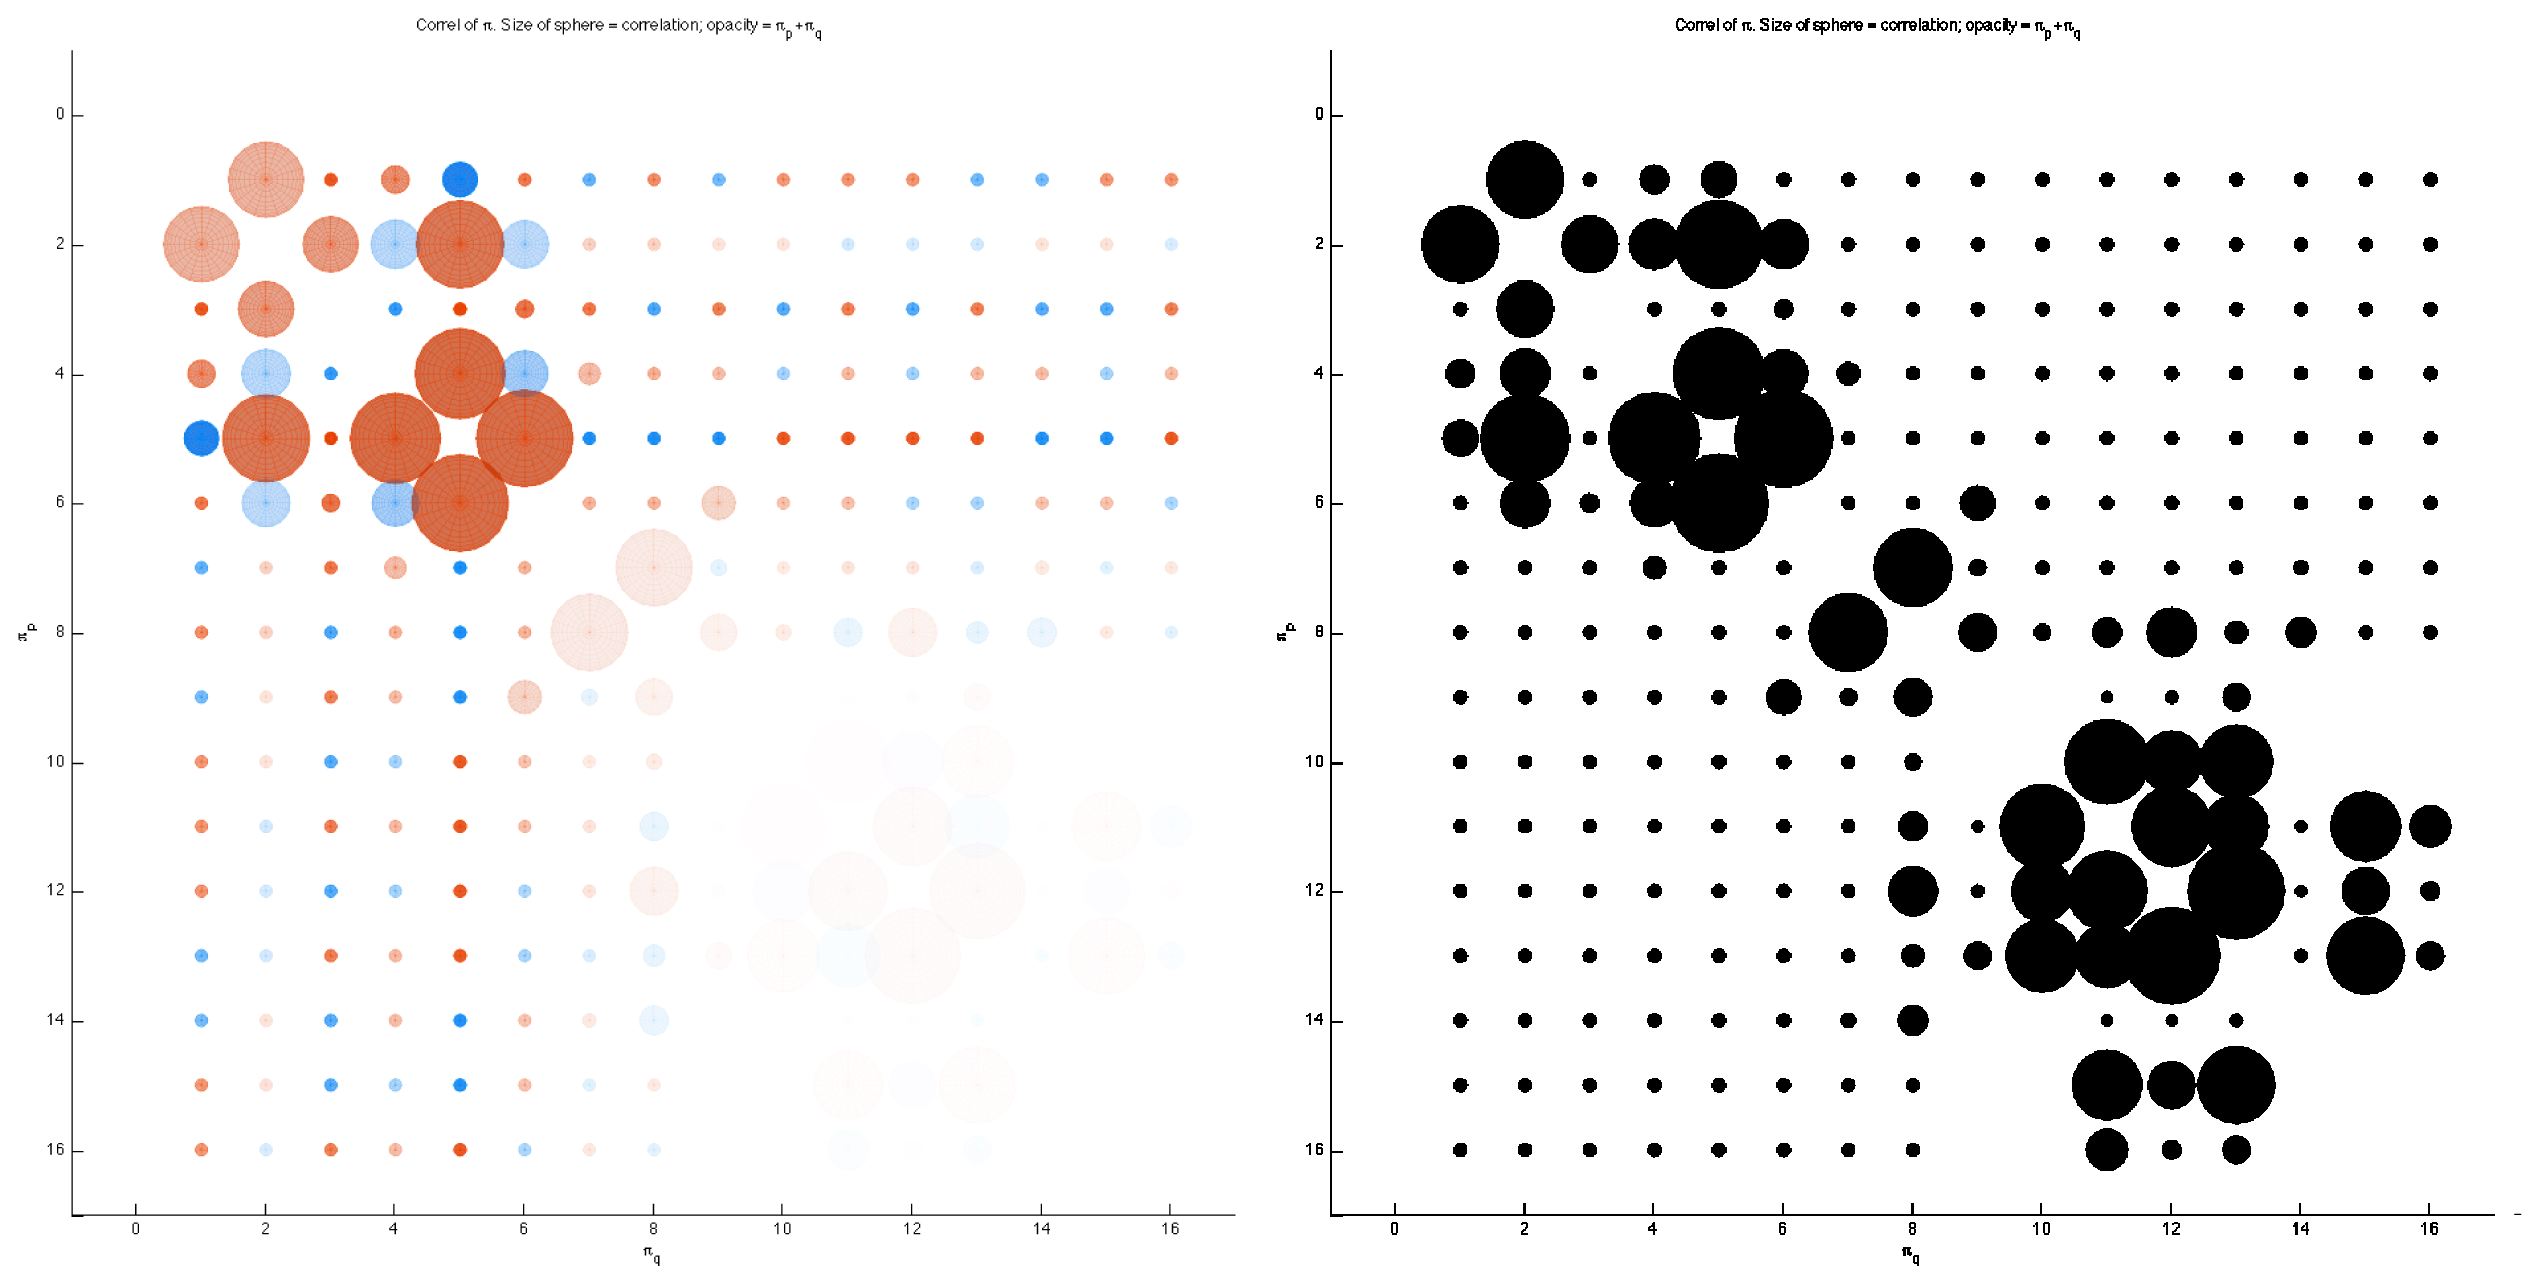
\includegraphics[scale=.75]{correlation_3.png}
	\end{center}
	\caption{Left: correlation where size of sphere represents correlation value, and opacity of sphere represents $\pi_q+\pi_p$. Orange bubbles represent negative correlation, and blue positive. Right: Same graph, but without transparency.}
\end{figure}




\begin{table}[h]\tiny
\caption{Correlation matrix}
	\begin{center}
		\noindent\makebox[\textwidth]{%
\begin{tabularx}{1.3\textwidth}{r| r r r r r r r r r r r r r r r r}
& 1 & 2 & 3 & 4 & 5 & 6 & 7 & 8 & 9 & 10 & 11 & 12 & 13 & 14 & 15 & 16	\\
\hline
   1   &    			             1   &    -0.592   &    -0.026   &    -0.219   &     0.274   &    -0.101   &     0.005   &    -0.008   &     0.007   &    -0.004   &    -0.003   &    -0.006   &     0.003   &     0.008   &    -0.001   &    -0.002     \\
   2   &    -0.592   &         1   &    -0.436   &     0.385   &    -0.685   &     0.378   &     -0.03   &    -0.006   &    -0.026   &    -0.003   &     0.002   &     0.002   &     0.003   &    -0.029   &    -0.004   &     0.006     \\
   3   &    -0.026   &    -0.436   &         1   &     0.074   &    -0.008   &    -0.141   &    -0.036   &     0.008   &    -0.006   &     0.004   &    -0.006   &     0.004   &    -0.008   &     0.025   &     0.002   &    -0.009     \\
   4   &    -0.219   &     0.385   &     0.074   &         1   &    -0.706   &     0.368   &    -0.173   &    -0.021   &    -0.045   &     0.013   &    -0.012   &     0.051   &    -0.022   &     -0.01   &     0.002   &    -0.003     \\
   5   &     0.274   &    -0.685   &    -0.008   &    -0.706   &         1   &    -0.757   &     0.057   &     0.008   &     0.083   &    -0.002   &         0   &    -0.018   &    -0.006   &     0.051   &     0.002   &    -0.001     \\
   6   &    -0.101   &     0.378   &    -0.141   &     0.368   &    -0.757   &         1   &    -0.012   &     -0.07   &    -0.264   &    -0.007   &     -0.01   &     0.027   &      0.02   &    -0.028   &    -0.009   &      0.01     \\
   7   &     0.005   &     -0.03   &    -0.036   &    -0.173   &     0.057   &    -0.012   &         1   &    -0.602   &     0.129   &    -0.013   &    -0.065   &    -0.023   &     0.025   &    -0.109   &     0.021   &    -0.002     \\
   8   &    -0.008   &    -0.006   &     0.008   &    -0.021   &     0.008   &     -0.07   &    -0.602   &         1   &     -0.29   &    -0.125   &     0.226   &    -0.381   &     0.173   &     0.232   &    -0.082   &     0.049     \\
   9   &     0.007   &    -0.026   &    -0.006   &    -0.045   &     0.083   &    -0.264   &     0.129   &     -0.29   &         1   &     0.112   &    -0.072   &     0.111   &    -0.211   &    -0.751   &     0.095   &    -0.048     \\
   10   &    -0.004   &    -0.003   &     0.004   &     0.013   &    -0.002   &    -0.007   &    -0.013   &    -0.125   &     0.112   &         1   &    -0.665   &     0.488   &    -0.567   &     0.091   &     0.439   &     -0.54     \\
   11   &    -0.003   &     0.002   &    -0.006   &    -0.012   &         0   &     -0.01   &    -0.065   &     0.226   &    -0.072   &    -0.665   &         1   &     -0.62   &     0.502   &    -0.044   &    -0.542   &     0.326     \\
   12   &    -0.006   &     0.002   &     0.004   &     0.051   &    -0.018   &     0.027   &    -0.023   &    -0.381   &     0.111   &     0.488   &     -0.62   &         1   &    -0.748   &    -0.006   &     0.376   &    -0.156     \\
   13   &     0.003   &     0.003   &    -0.008   &    -0.022   &    -0.006   &      0.02   &     0.025   &     0.173   &    -0.211   &    -0.567   &     0.502   &    -0.748   &         1   &     0.015   &    -0.599   &     0.218     \\
   14   &     0.008   &    -0.029   &     0.025   &     -0.01   &     0.051   &    -0.028   &    -0.109   &     0.232   &    -0.751   &     0.091   &    -0.044   &    -0.006   &     0.015   &         1   &     0.008   &    -0.248     \\
   15   &    -0.001   &    -0.004   &     0.002   &     0.002   &     0.002   &    -0.009   &     0.021   &    -0.082   &     0.095   &     0.439   &    -0.542   &     0.376   &    -0.599   &     0.008   &         1   &    -0.382     \\
   16   &    -0.002   &     0.006   &    -0.009   &    -0.003   &    -0.001   &      0.01   &    -0.002   &     0.049   &    -0.048   &     -0.54   &     0.326   &    -0.156   &     0.218   &    -0.248   &    -0.382   &         1     \\

\end{tabularx}}
	\end{center}
\end{table}




\begin{figure}
	
	\begin{center}
		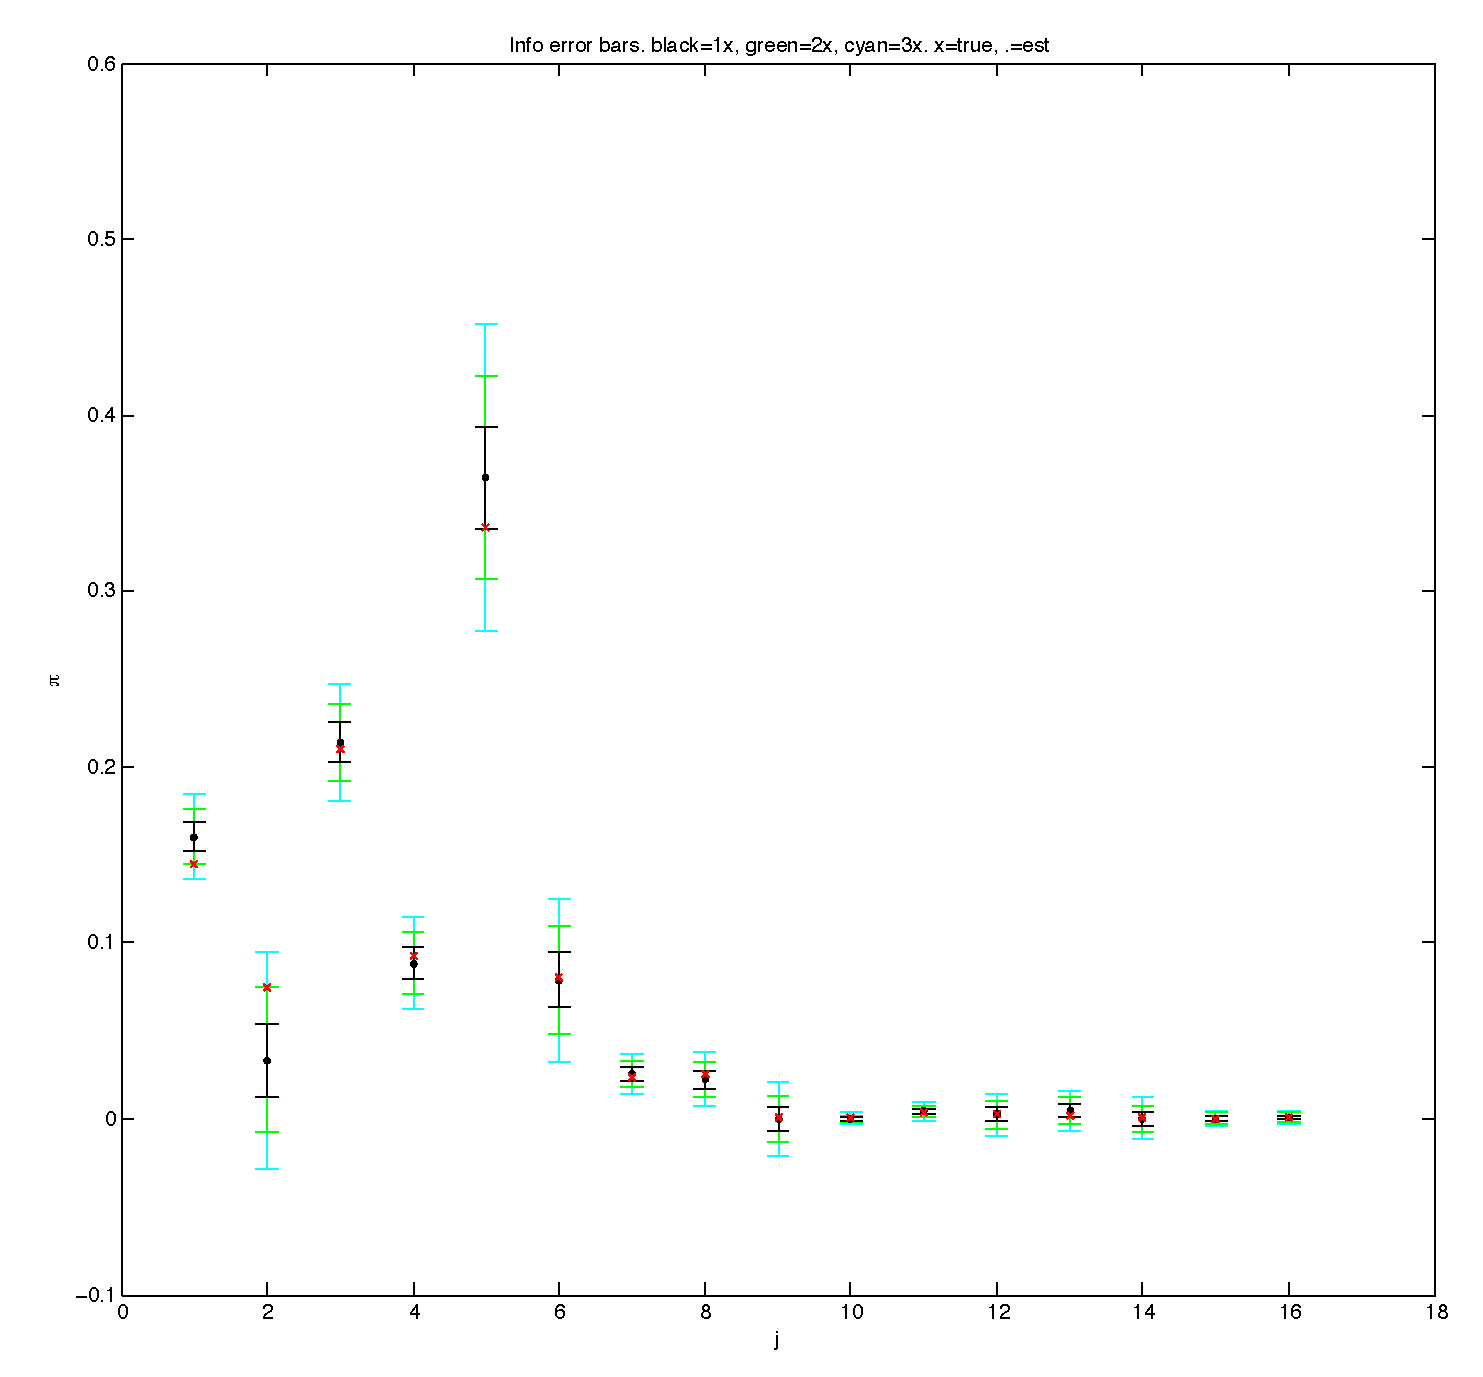
\includegraphics[scale=0.6]{info_error_bars.pdf}
	\end{center}
	\caption{$\vp$ plus information based error bars for $\pm \sigma$ (black), $\pm 2\sigma$ (green), and $\pm 3\sigma$ (cyan). A red $\times$ represents the true value, and a black dot represents the estimated values, $\vph$.}
\end{figure}


\begin{figure}
	
	\begin{center}
		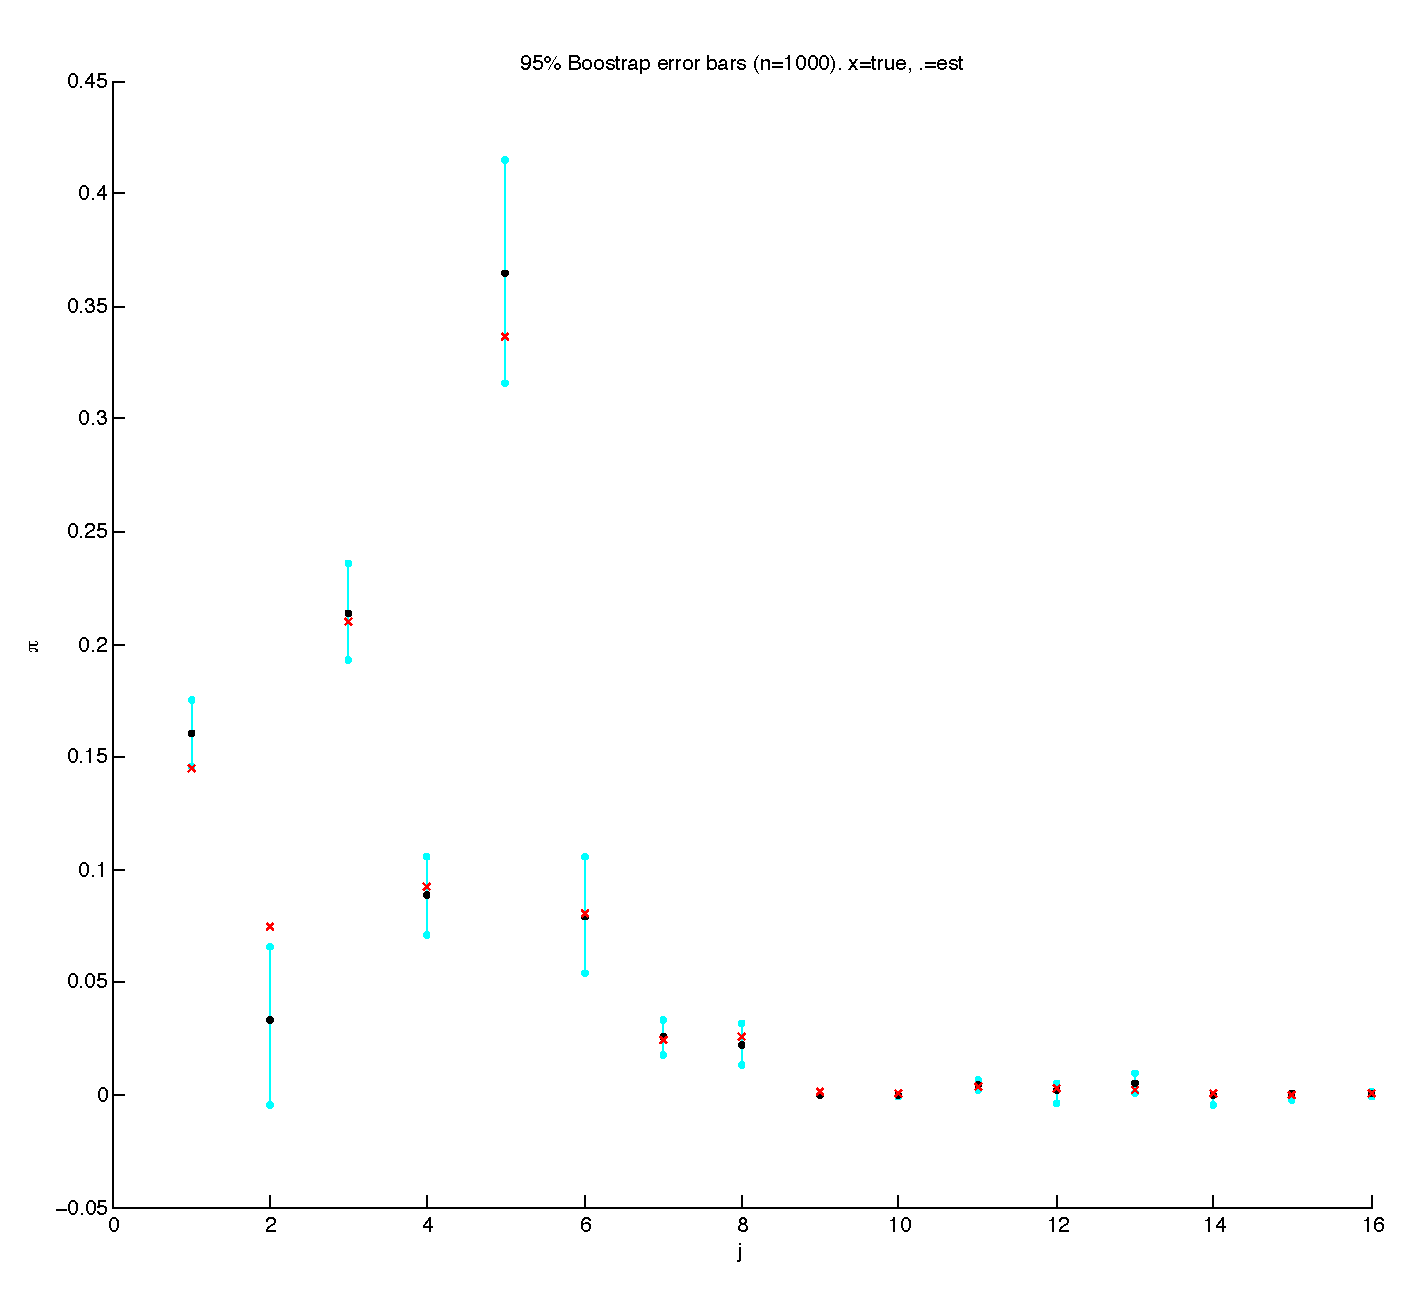
\includegraphics[scale=0.6]{boot_mn_error_bars.pdf}
	\end{center}
	\caption{M-out-of n bootstrapped confidence intervals for $\vp$. A red $\times$ represents the true value, and a black dot represents the estimated values, $\vph$.}
\end{figure}


\begin{figure}
	
	\begin{center}
		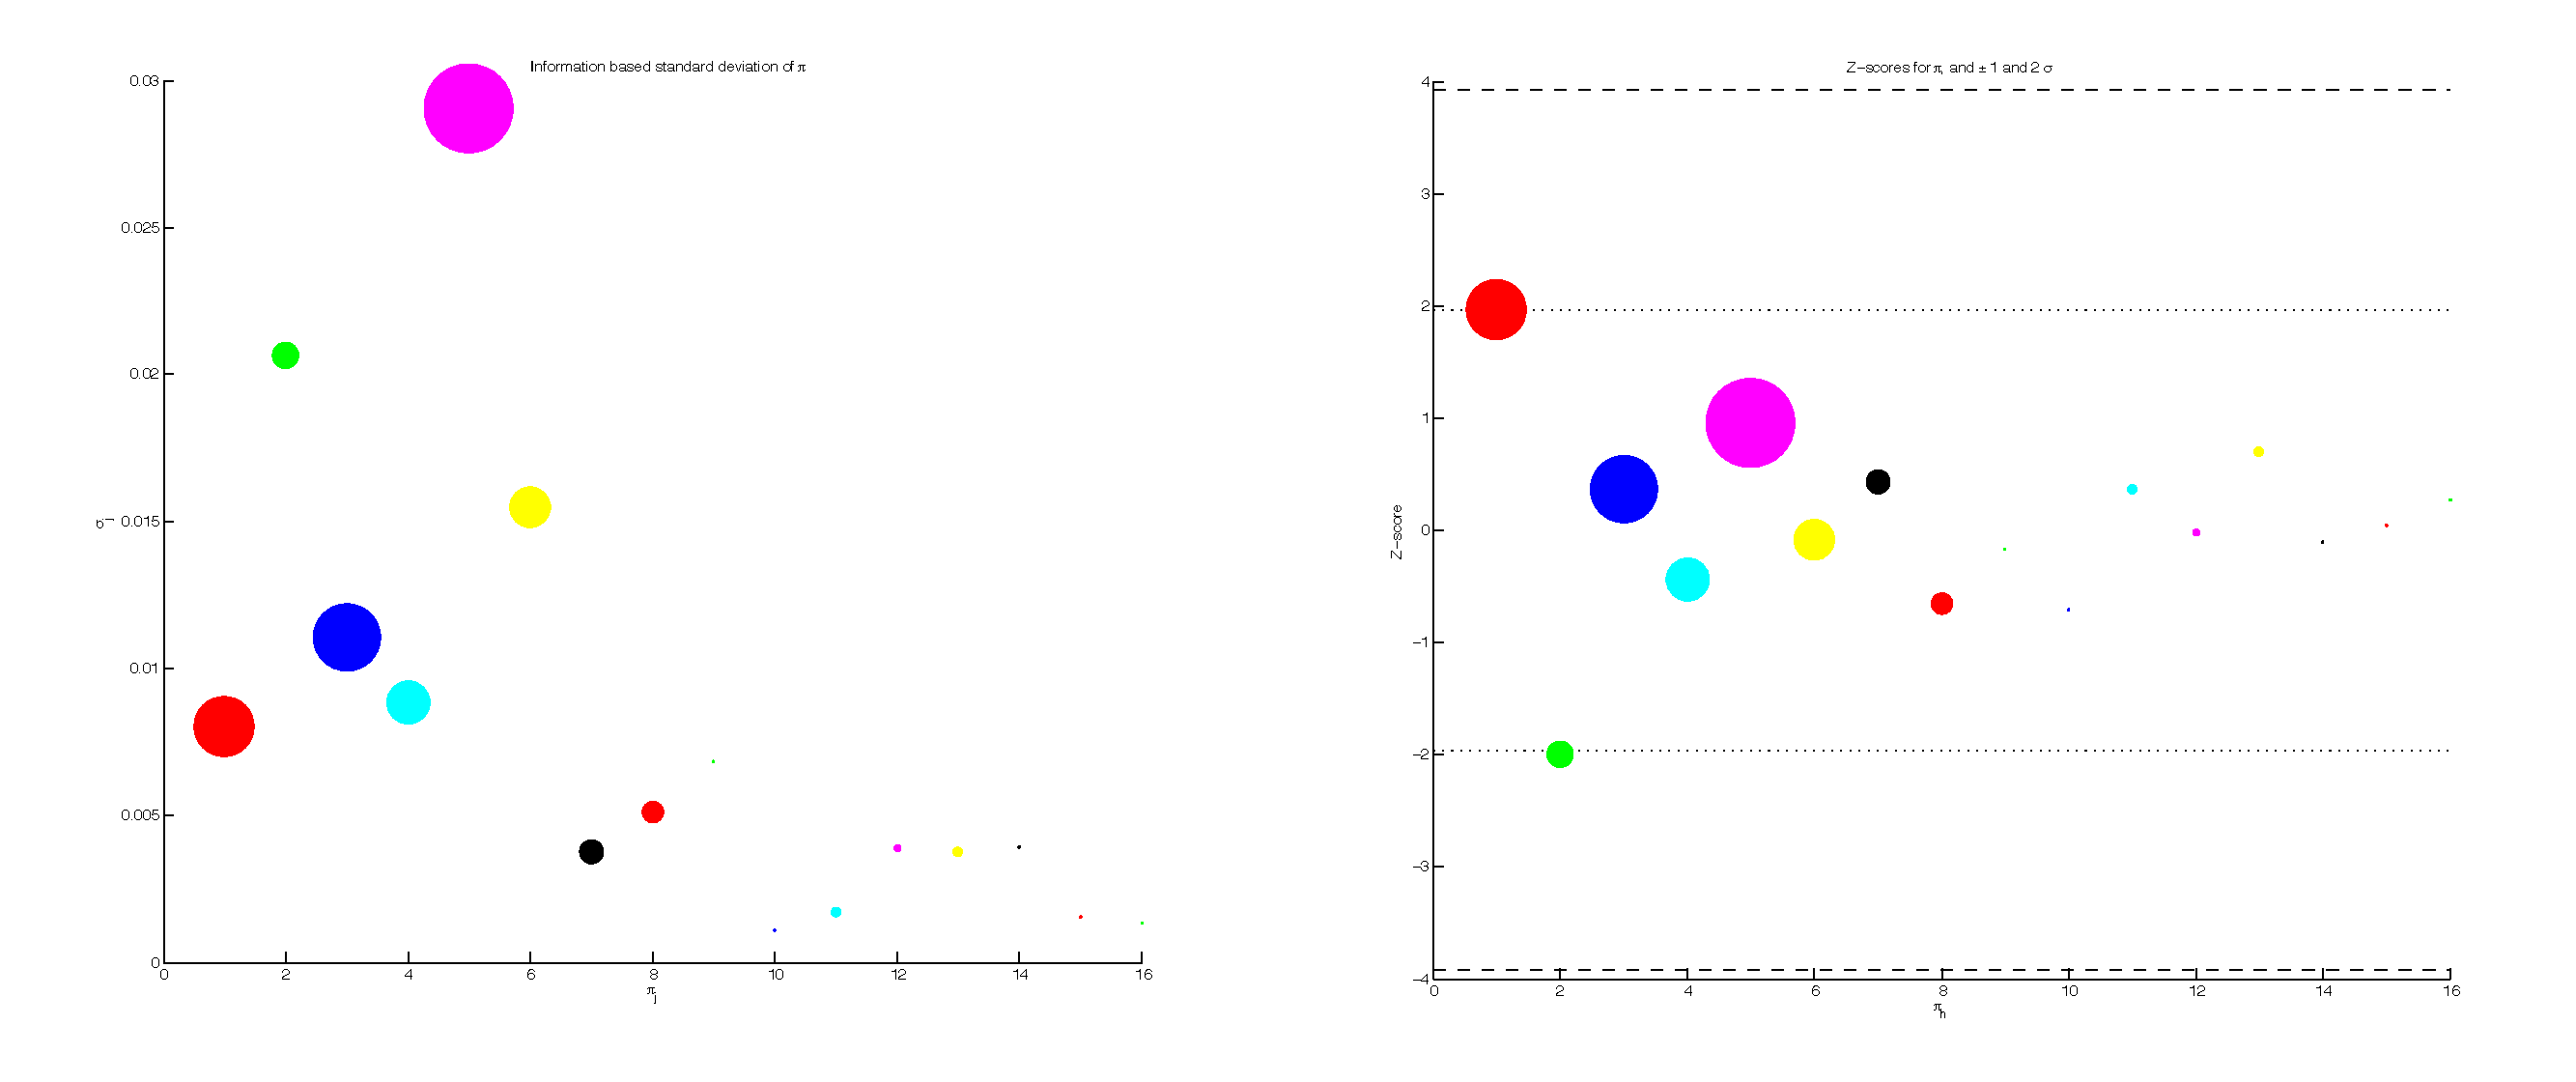
\includegraphics[scale=0.5]{zsc.pdf}
	\end{center}
	\caption{Left: standard deviation of each $\pi_j$. Right: Z-score, with 1 and 2 standard deviations marked as dotted lines. Colors are same as EM diagnostic plots. Size represents the value of $\pi_j$.}
\end{figure}

\begin{figure}

\begin{tabular}{r| r| r| r| r|}
		& $\hat{\pi}_j$ & $\pi_j$ & Std. dev. & Z-score	\\
		\hline
1	& 16.04   &     14.47   &         0.0080    &    1.965      \\
2	&  3.32   &      7.44   &         0.0206   &   -1.995      \\
3	& 21.39   &     20.99   &         0.0110   &    0.363      \\
4	&  8.85   &      9.23   &         0.0088    &   -0.439      \\
5	& 36.44   &     33.66   &         0.0290   &     0.96      \\
6	&  7.88   &      8.02   &         0.0154   &   -0.088      \\
7	&  2.56   &       2.4   &         0.0037    &    0.428      \\
8	&  2.24   &      2.57   &         0.0051    &   -0.655      \\
9	&     0   &      0.12   &         0.0068    &   -0.174      \\
10	&     0   &      0.08   &         0.0010    &   -0.706      \\
11	&  0.42   &      0.36   &         0.0017   &    0.367      \\
12	&  0.25   &      0.25   &         0.0038    &   -0.016      \\
13	&  0.49   &      0.23   &         0.0037    &    0.694      \\
14	&  0.01   &      0.05   &         0.0039    &   -0.103      \\
15	&  0.03   &      0.02   &         0.0015    &    0.044      \\
16	&  0.08   &      0.05   &         0.0013    &     0.27      \\   		\end{tabular}
\caption{Model 3 EM results}
\end{figure}
               

%%%%%%%%%%%%%%%%%%%%%%%%%%%%%%%%%%%%%%%%%%%%%%%%%%%%%%
\clearpage
\section{Likelihood ratio test}
Given certain regularity conditions, let
\eqn{
	H_0: \vp = \vp_\text{true}	\\
	H_1: \vp \neq \vp_\text{true}
}

The likelihood ratio test is then
\eqn{
	\Lambda = -2 \log \frac{ \sup_{\vp=\vp_\text{true}} \llp}{ \sup_{\vp} \llp }  = -2\bl l(\vp_\text{true}) - l(\vph) \br \sim \chi^2_{m-1}	\\
}

For halo 3,
\eqn{
	\Lambda_\text{Halo 3} &= 25.025 \sim \chi^2_{15}	\\
	\text{p-value 10k} &= 4.961\%\\
	\text{p-value 30k} &= 1.3\times 10^{-5}\%\\
	\text{p-value 50k} &= 1.4\times 10^{-12}\%
}

Thus we accept $H_0$ when requiring 95\% or less confidence; there is only a 4.961\% chance we would see a value this extreme or more given $H_0$ is true. This holds for 400 to 1600 EM iterations.






\end{document}











%%%%%%%%%%%%%%%%%%%%%%%%%%%%%%%%%%%%%%%%%%%%%%%%%%%%%%
\clearpage
\section{Other}
\subsection{Convergence}
$\llp$ from 1.235 to 1.236 over past 25 runs is the slowest rate of convergence.

\subsection{To do}
Bias, consistency, efficiency, method of moments, $\sigma$ as a function of n. Bootstrapping, n+1 bootstrapping as a check that n is large enough for fisher info.


MAP 2.8.5.

Alt T 2.7.3.

basis of test 2.7.1.

deterministic annealing em algo 2.12.4.

stochiastic em 2.13.

conditional bootstrap 2.15.5. 


alt approach to fisher info: 2.16.1: using wald and reduced parameter holding out.

full bootstrap 2.16.2



2.18.2 modified lrt

2.18.1 outliers

2.19 partial classification

3.5

3.8.1


spectral decomposition: 3.12.1

k means classification for auto binning?

4: mcmc for mixture

5.5.2: exactly what we did--nonormal

5.5.4: mulitcycle

5.13 hierarchical mixtures of experts


6.13 skewness of lrt and m

6.3.2

6.5

6.6 bootstrapping lrts

6.7 pval boots

6.7.2 double boots

6.8 bias corr for log like, aic, boots info, cv info

6.9 bayeseian info

6.10 classification based info

9 fitting mix to bin data

11 mix analys of directional data

13 hidden markov models
















